\documentclass{article}
\usepackage[utf8]{inputenc}
% are all of these packages really necessary?
% no.
% i'm just too lazy to only grab the packages i want for a specific
% document, so i just glob all of my most commonly used packages together
% this is bad practice.
\usepackage{amsmath,amsthm,amssymb,amsfonts, fancyhdr, color, comment, graphicx, environ, mdframed, soul, calc, enumitem, mdframed, xcolor, geometry, empheq, mathtools, tikz, pgfplots, caption, subcaption}

\usetikzlibrary{external}
\tikzexternalize[prefix=tikz/,optimize command away=\includepdf]

%tikzpicture
\usepackage{tikz}
\usepackage{scalerel}
\usepackage{pict2e}
\usepackage{tkz-euclide}
\usetikzlibrary{calc}
\usetikzlibrary{patterns,arrows.meta}
\usetikzlibrary{shadows}
\usetikzlibrary{external}

%pgfplots
\usepackage{pgfplots}
\pgfplotsset{compat=newest}
\usepgfplotslibrary{statistics}
\usepgfplotslibrary{fillbetween}
\usepgfplotslibrary{polar}

\tikzset{external/export=true}
\pgfplotsset{
    standard/.style={
    axis line style = thick,
    trig format=rad,
    enlargelimits,
    axis x line=middle,
    axis y line=middle,
    enlarge x limits=0.15,
    enlarge y limits=0.15,
    every axis x label/.style={at={(current axis.right of origin)},anchor=north west},
    every axis y label/.style={at={(current axis.above origin)},anchor=south east}
    }
}
\newcommand*\widefbox[1]{\fbox{\hspace{2em}#1\hspace{2em}}}
% Command "alignedbox{}{}" for a box within an align environment
% Source: http://www.latex-community.org/forum/viewtopic.php?f=46&t=8144
\newlength\dlf  % Define a new measure, dlf
\newcommand\alignedbox[2]{
% Argument #1 = before & if there were no box (lhs)
% Argument #2 = after & if there were no box (rhs)
&  % Alignment sign of the line
{
\settowidth\dlf{$\displaystyle #1$}  
    % The width of \dlf is the width of the lhs, with a displaystyle font
\addtolength\dlf{\fboxsep+\fboxrule}  
    % Add to it the distance to the box, and the width of the line of the box
\hspace{-\dlf}  
    % Move everything dlf units to the left, so that & #1 #2 is aligned under #1 & #2
\boxed{#1 #2}
    % Put a box around lhs and rhs
}
}

\newcommand{\lrp}[1]{\left( #1 \right)}
\newcommand{\abs}[1]{\left\vert #1 \right\vert}
\newcommand{\lra}[1]{\left\langle #1 \right\rangle}
\newcommand{\lrb}[1]{\left[ #1 \right]}
\newcommand{\iintR}[0]{\iint\limits_{R}}

\geometry{letterpaper, portrait, margin=1in}
\renewcommand{\footrulewidth}{0.8pt}
\setlength\parindent{0pt}
\pagestyle{fancy}
\lhead{Christina Phan}
\rhead{MAT 21D} 
\chead{\textbf{Homework 5 Solutions}}

\newcommand{\Solution}{\textit{Solution}}
\pgfplotsset{compat=1.18}
\begin{document}
\textbf{Note}

For most of the problems, I omitted a few integration steps. If you need help, feel free to PM me, or go to OH.

\textbf{Problem 1}

Find the centroid of the region:

\textbf{(a)} The triangular region cut from the first quadrant by the line $x+y=3$.

\Solution

The centroid is the point $\displaystyle \lrp{\overline{x},\overline{y}}$.

To get $\overline{x}$ and $\overline{y}$, we'll need to know $M$, $M_x$, and $M_y$.

For $M$,

Let's graph the triangular region. 
\begin{center}
\resizebox{3.5cm}{!}{
    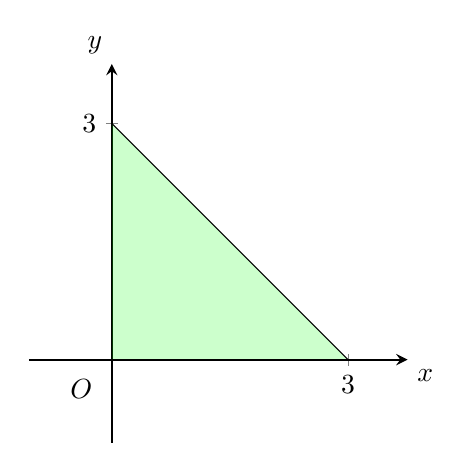
\begin{tikzpicture}
    \begin{axis}[standard,
            xtick={3},
            ytick={3},
            samples=1000,
            xlabel={$x$},
            ylabel={$y$},
            xmin=-0.5,xmax=3.2,
            ymin=-0.5,ymax=3.2,
            x=1cm,
            y=1cm/1,
           ]
\node[anchor=center,label=south west:$O$] at (axis cs:0,0){};
\addplot[name path=F,domain={0:3}]{3-x};
\addplot[name path=G, domain={0:3}]{0};
\addplot[fill=green, fill opacity=0.2] fill between [of=F and G, soft clip={domain=0:3}];
    \end{axis}
    \end{tikzpicture}
}
\end{center} 
In terms of $x$, the lower $y$ bound is $0$ and the upper $y$ bound is $y=3-x$. The lower $x$ bound is $0$ and the upper $x$ bound is $3$.
\begin{align*}
    M&=\int_0^3\int_0^{3-x}\,dy\,dx\\
    &=\int_0^3\lrb{y}_0^{3-x}\,dx\\
    &=\int_0^3 3-x\,dx\\
    &=\lrb{3x-\frac{1}{2}x^2}_0^3\\
    &=3(3)-\frac{1}{2}(3)^2\\
    &=\frac{9}{2}
\end{align*}

For $M_x$,

The region bounds will remain the same as the region bounds for $M$.
\begin{align*}
    M_x&=\int_0^3\int_0^{3-x}y\,dy\,dx\\
    &=\int_0^3 \lrb{\frac{1}{2}y^2}_0^{3-x}\\
    &=\int_0^3 \frac{1}{2}(3-x)^2\,dx\\
    &=\lrb{-\frac{1}{4}(3-x)^2}_0^3\\
    &=\lrp{-\frac{1}{6}(3-3)^3}-\lrp{-\frac{1}{6}(3-0)^3}\\
    &=\frac{9}{2}
\end{align*}

For $M_y$,

The region bounds will remain the same as the region bounds for $M$.
\begin{align*}
    M_y&=\int_0^3\int_0^{3-x}x\,dy\,dx\\
    &=\int_0^3\lrb{xy}_0^{3-x}\,dx\\
    &=\int_0^3 x(3-x)\,dx\\
    &=\int_0^3 3x-x^2\,dx\\
    &=\lrb{\frac{3}{2}x^2-\frac{1}{3}x^3}_0^3\\
    &=\frac{3}{2}(3)^2-\frac{1}{3}(3)^3\\
    &=\frac{9}{2}
\end{align*}
Our final answer is
\begin{subequations}
    \begin{empheq}[box=\widefbox]{align}
        \overline{x}&=\frac{M_y}{M}=\frac{\frac{9}{2}}{\frac{9}{2}}=1\nonumber\\
        \overline{y}&=\frac{M_x}{M}=\frac{\frac{9}{2}}{\frac{9}{2}}=1\nonumber\\
        \text{centroid:}&
        \lrp{1,1}\nonumber
    \end{empheq}
\end{subequations}
\textbf{(b)} The region between the $x$-axis and the arch $y=\sin x$.

\Solution

We will assume that this region is in the first quadrant, and is when $y$ hits the $x$-axis first.

The centroid is the point $\displaystyle \lrp{\overline{x},\overline{y}}$.

To get $\overline{x}$ and $\overline{y}$, we'll need to know $M$, $M_x$, and $M_y$.

For $M$,

Let's graph the region. 
\begin{center}
\resizebox{3.5cm}{!}{
    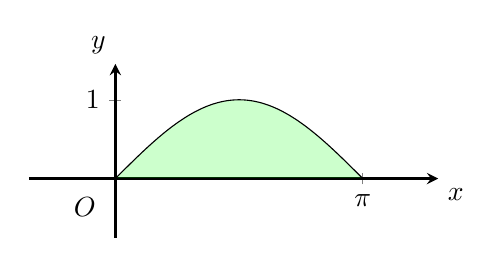
\begin{tikzpicture}
    \begin{axis}[standard,
            xtick={3.14159},
            ytick={1},
            samples=1000,
            xlabel={$x$},
            ylabel={$y$},
            xmin=-0.5,xmax=3.5,
            ymin=-0.5,ymax=1.2,
            x=1cm,
            y=1cm/1,
            xticklabels={$\pi$}
           ]
\node[anchor=center,label=south west:$O$] at (axis cs:0,0){};
\addplot[name path=F,domain={0:3.14159}]{sin(x)};
\addplot[name path=G, domain={0:3.14159}]{0};
\addplot[fill=green, fill opacity=0.2] fill between [of=F and G, soft clip={domain=0:3.14159}];
    \end{axis}
    \end{tikzpicture}
}
\end{center}
In terms of $x$, the lower $y$ bound is $0$ and the upper $y$ bound is $y=\sin x$. The lower $x$ bound is $0$ and the upper $x$ bound is $\pi$.
\begin{align*}
    M&=\int_0^\pi\int_0^{\sin x}\,dy\,dx\\
    &=\int_0^\pi \lrb{y}_0^{\sin x}\,dx\\
    &=\int_0^\pi \sin x\,dx\\
    &=\lrb{-\cos x}_0^\pi\\
    &=(1)-(-1)\\
    &=2
\end{align*}
For $M_x$,

The region bounds will remain the same as the region bounds for $M$.
\begin{align*}
    M_x&=\int_0^\pi\int_0^{\sin x}y\,dy\,dx\\
    &=\int_0^\pi \lrb{\frac{1}{2}y^2}_0^{\sin x}\,dx\\
    &=\int_0^\pi \frac{1}{2}\sin^2 x\,dx\\
    &=\frac{1}{2}\int_0^\pi\frac{1}{2} \lrp{1-\cos 2x}\,dx\tag{$\sin^2 x=\frac{1}{2}(1-\cos 2x)$}\\
    &=\frac{1}{4}\int_0^\pi 1-\cos 2x\,dx\\
    &=\frac{1}{4}\lrb{x-\frac{1}{2}\sin 2x}_0^{\pi}\\
    &=\frac{1}{4}\lrp{\pi-\frac{1}{2}(0)}\\
    &=\frac{\pi}{4}
\end{align*}
For $M_y$,

The region bounds will remain the same as the region bounds for $M$.
\begin{align*}
    M_y&=\int_0^\pi \int_0^{\sin x}x\,dy\,dx\\
    &=\int_0^\pi \lrb{xy}_0^{\sin x}\,dx\\
    &=\int_0^\pi x\sin x\,dx\\
    &u=x\hspace{2em}dv=\sin x\,dx\\
    &du=dx\hspace{2em}v=-\cos x\\
    &=\lrb{-x\cos x}_0^\pi+\int_0^\pi \cos x\,dx\\
    &=\lrp{-\pi \cos \pi}+\lrb{\sin x}_0^\pi\\
    &=\pi +(0-0)\\
    &=\pi
\end{align*}
Our final answer is
\begin{subequations}
    \begin{empheq}[box=\widefbox]{align}
        \overline{x}&=\frac{M_y}{M}=\frac{\pi}{2}\nonumber\\
        \overline{y}&=\frac{M_x}{M}=\frac{\frac{\pi}{4}}{2}=\frac{\pi}{8}\nonumber\\
        \text{centroid:}&
        \lrp{\frac{\pi}{2},\frac{\pi}{8}}\nonumber
    \end{empheq}
\end{subequations}
\textbf{(c)} The infinite region in the second quadrant enclosed by the coordinate axes and
the curve $y=e^x$.

\Solution

The centroid is the point $\displaystyle \lrp{\overline{x},\overline{y}}$.

To get $\overline{x}$ and $\overline{y}$, we'll need to know $M$, $M_x$, and $M_y$.

For $M$,

Let's graph the region.
\begin{center}
\resizebox{3.5cm}{!}{
    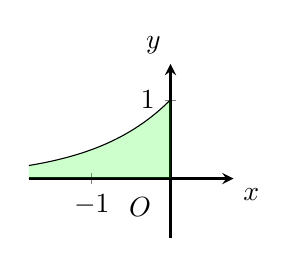
\begin{tikzpicture}
    \begin{axis}[standard,
            xtick={-1},
            ytick={1},
            samples=1000,
            xlabel={$x$},
            ylabel={$y$},
            xmin=-1.5,xmax=0.5,
            ymin=-0.5,ymax=1.2,
            x=1cm,
            y=1cm/1,
           ]
\node[anchor=center,label=south west:$O$] at (axis cs:0,0){};
\addplot[name path=F,domain={-2:0}]{e^x};
\addplot[name path=G, domain={-2:0}]{0};
\addplot[fill=green, fill opacity=0.2] fill between [of=F and G,soft clip={domain=-2:0}];
    \end{axis}
    \end{tikzpicture}
}
\end{center}
In terms of $x$, the lower $y$ bound is $0$ and the upper $y$ bound is $y=e^x$. The lower $x$ bound is $-\infty$ and the upper $x$ bound is $0$.
\begin{align*}
  M&=\int_{-\infty}^0\int_0^{e^x}\,dy\,dx\\
  &=\int_{-\infty}^0 \lrb{y}_0^{e^x}\,dx\\
  &=\int_{-\infty}^0 e^x\,dx\\
  &=\lim_{t\to-\infty}\int_{t}^0 e^x\,dx\\
  &=\lim_{t\to-\infty}\lrb{e^x}_t^0\\
  &=\lim_{t\to-\infty} 1-e^t\\
  &=1
\end{align*}
For $M_x$,

The region bounds will remain the same as the region bounds for $M$.
\begin{align*}
    M_x&=\int_{-\infty}^0\int_0^{e^x} y\,dy\,dx\\
    &=\int_{-\infty}^0 \lrb{\frac{1}{2}y^2}_0^{e^x}\,dx\\
    &=\int_{-\infty}^0 \frac{1}{2}e^{2x}\,dx\tag{$\lrp{e^x}^2=e^{2x}$}\\
    &=\lim_{t\to-\infty}\int_{t}^0 \frac{1}{2}e^{2x}\,dx\\
    &=\lim_{t\to-\infty}\lrb{\frac{1}{4}e^{2x}}_t^0\\
    &=\lim_{t\to-\infty} \frac{1}{4} - e^{2t}\\
    &=\frac{1}{4}
\end{align*}
For $M_y$,

The region bounds will remain the same as the region bounds for $M$.
\begin{align*}
   M_y &=\int_{-\infty}^0\int_0^{e^x} x\,dy\,dx\\
   &=\int_{-\infty}^0 \lrb{xy}_0^{e^x}\,dx\\
   &=\int_{-\infty}^0 xe^x \,dx\\
   &=\lim_{t\to-\infty}\int_t^0 xe^x\,dx\\
   &u=x\hspace{2em}dv=e^x\,dx\\
   &du=dx\hspace{2em}v=e^x\\
   &=\lim_{t\to-\infty} \lrb{xe^x}_t^0-\int_t^0 e^x\,dx\\
   &=\lim_{t\to-\infty} \lrp{0-te^t}-\lrb{e^x}_t^0\\
   &=\lim_{t\to-\infty} -te^t - \lrp{1-e^t}\\
   &= 0 - 1 + 0\\
   &=-1
\end{align*}
Our final answer is
\begin{subequations}
    \begin{empheq}[box=\widefbox]{align}
        \overline{x}&=\frac{M_y}{M}=\frac{-1}{1}=-1\nonumber\\
        \overline{y}&=\frac{M_x}{M}=\frac{\frac{1}{4}}{1}=\frac{1}{4}\nonumber\\
        \text{centroid:}&
        \lrp{-1,\frac{1}{4}}\nonumber
    \end{empheq}
\end{subequations}
\textbf{Problem 2} 

Find the mass of a plate occupying the smaller region cut from the ellipse $x^2+ 4y^2= 12$
by the parabola $x=4y^2$ if $\delta(x,y)=5x$.

\Solution

Let's graph the region. 
\begin{center}
\resizebox{3.5cm}{!}{
    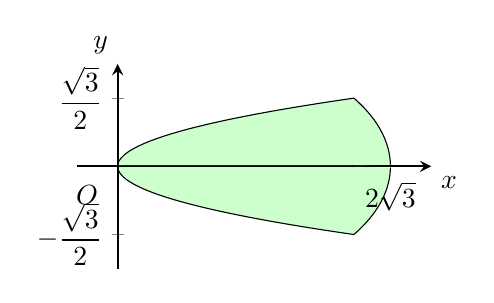
\begin{tikzpicture}
    \begin{axis}[standard,
            xtick={3.464},
            ytick={-0.866,0.866},
            samples=1000,
            xlabel={$x$},
            ylabel={$y$},
            xmin=0,xmax=3.464,
            ymin=-1,ymax=1,
            x=1cm,
            y=1cm/1,
            xticklabels={$2\sqrt{3}$},
            yticklabels={$-\dfrac{\sqrt{3}}{2}$,$\dfrac{\sqrt{3}}{2}$},
           ]
\node[anchor=center,label=south west:$O$] at (axis cs:0,0){};
\addplot[name path=F,domain={3:3.464}]{sqrt(3-0.25*x^2)};
\addplot[name path=G,domain={3:3.464}]{-sqrt(3-0.25*x^2)};
\addplot[name path=H,domain={0:3}]{sqrt(0.25*x)};
\addplot[name path=I,domain={0:3}]{-sqrt(0.25*x)};
\addplot[name path=J, domain={0:3}]{0};
\addplot[fill=green, fill opacity=0.2] fill between [of=F and J,soft clip={domain=3:3.464}];
\addplot[fill=green, fill opacity=0.2] fill between [of=G and J,soft clip={domain=3:3.464}];
\addplot[fill=green, fill opacity=0.2] fill between [of=H and J,soft clip={domain=0:3}];
\addplot[fill=green, fill opacity=0.2] fill between [of=I and J,soft clip={domain=0:3}];
    \end{axis}
    \end{tikzpicture}
}
\end{center}

We can find the $y$ value of the intersection point if we use the equation $x=4y^2$ in the equation $x^2+4y^2=12$.
\begin{align*}
    (4y^2)^2+4y^2&=12\\
    16y^4+4y^2-12&=0\\
    4y^4+y^2-3&=0\\
    (4y^2 - 3)(y^2 +1)&=0\\
    4y^2&=3\tag{$y^2+1=0$ makes imaginary solutions}\\
    y&=\pm\frac{\sqrt{3}}{2}
\end{align*}
In terms of $y$, our lower bounds for $x$ is $x=4y^2$ and our upper bounds for $x$ is $x=\sqrt{12-4y^2}$. Our lower bounds for $y$ is $\displaystyle -\frac{\sqrt{3}}{2}$ and our upper bounds for $y$ is $\displaystyle \frac{\sqrt{3}}{2}$.
\begin{align*}
    M&=\int_{-\frac{\sqrt{3}}{2}}^{\frac{\sqrt{3}}{2}}\int_{4y^2}^{\sqrt{12-4y^2}}5x\,dx\,dy\\
    &=\int_{-\frac{\sqrt{3}}{2}}^{\frac{\sqrt{3}}{2}}\lrb{\frac{5}{2}x^2}_{4y^2}^{\sqrt{12-4y^2}}\,dy\\
    &=\int_{-\frac{\sqrt{3}}{2}}^{\frac{\sqrt{3}}{2}} \frac{5}{2}(12-4y^2)-\frac{5}{2}(4y^2)^2\,dy\\
    &=\int_{-\frac{\sqrt{3}}{2}}^{\frac{\sqrt{3}}{2}}30-10y^2-40y^4\,dy\\
    &=\lrb{30y-\frac{10}{3}y^3-8y^5}_{-\frac{\sqrt{3}}{2}}^{\frac{\sqrt{3}}{2}}\\
    &=\lrp{30\lrp{\frac{\sqrt{3}}{2}}-\frac{10}{3}\lrp{\frac{\sqrt{3}}{2}}^3-8\lrp{\frac{\sqrt{3}}{2}}^5}-\lrp{30\lrp{-\frac{\sqrt{3}}{2}}-\frac{10}{3}\lrp{-\frac{\sqrt{3}}{2}}^3-8\lrp{\frac{-\sqrt{3}}{2}}^5}\\
    &=\boxed{23\sqrt{3}}\tag{use your calculator :)}
\end{align*}
\textbf{Problem 3}

Find the center of mass:

\textbf{(a)} A triangular plate bounded by the $y$-axis and the lines $y = x$ and $y = 2 -x$ if
$\delta(x,y) = 6x + 3y + 3$.

\Solution

Let's graph the region.
\begin{center}
\resizebox{3.5cm}{!}{
    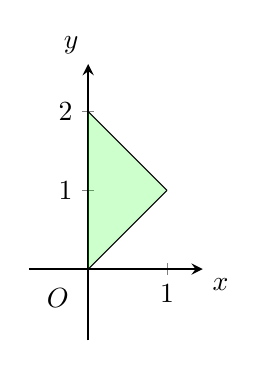
\begin{tikzpicture}
    \begin{axis}[standard,
            xtick={1,2},
            ytick={1,2},
            samples=1000,
            xlabel={$x$},
            ylabel={$y$},
            xmin=-0.5,xmax=1.2,
            ymin=-0.5,ymax=2.2,
            x=1cm,
            y=1cm/1
           ]
\node[anchor=center,label=south west:$O$] at (axis cs:0,0){};
\addplot[name path=F,domain={0:1}]{-x+2};
\addplot[name path=G,domain={0:1}]{x+0};
\addplot[fill=green, fill opacity=0.2] fill between [of=F and G,soft clip={domain=0:1}];
    \end{axis}
    \end{tikzpicture}
}
\end{center}
In terms of $x$, our lower bound for $y$ is $y=x$ and our upper bound for $y$ is $y=2-x$. Our lower bound for $x$ is $x=0$ and our upper bound for $x$ is $x=1$.

For $M$,
\begin{align*}
    M&=\int_0^1\int_x^{2-x}6x+3y+3\,dy\,dx\\
    &=\int_0^1\lrb{6xy+\frac{3}{2}y^2+3y}_x^{2-x}\,dx\\
    &=\int_0^1 12 -12x^2\,dx\tag{lots of algebra here...}\\
    &=\lrb{12x-4x^3}_0^1\\
    &=8
\end{align*}
For $M_x$,

Our region bounds are the same as the region bounds for $M$.
\begin{align*}
    M_x&=\int_0^1\int_x^{2-x} y(6x+3y+3)\,dy\,dx\\
    &=\int_0^1\int_x^{2-x} 6xy+3y^2+3y\,dy\,dx\\
    &=\int_0^1 \lrb{3xy^2+y^3+\frac{3}{2}y^2}_x^{2-x}\,dx\\
    &=\int_0^1 14-6x-6x^2-2x^3\,dx\tag{lots of algebra here...}\\
    &=\lrb{14x-3x^2-2x^3-\frac{1}{2}x^4}_0^1\\
    &=\frac{17}{2}
\end{align*}
For $M_y$,

Our region bounds are the same as the region bounds for $M$.
\begin{align*}
    M_y&=\int_0^1\int_x^{2-x} x(6x+3y+3)\,dy\,dx\\
    &=\int_0^1\int_x^{2-x} 6x^2+3xy+3x\,dy\,dx\\
    &=\int_0^1\lrb{6x^2y+\frac{3}{2}xy^2+3xy}_x^{2-x}\,dx\\
    &=\int_0^1 12x-12x^3\,dx\tag{lots of algebra here...}\\
    &=\lrb{6x^2-3x^4}_0^1\\
    &=3
\end{align*}
Our final answer is
\begin{subequations}
    \begin{empheq}[box=\widefbox]{align}
        \overline{x}&=\frac{M_y}{M}=\frac{3}{8}\nonumber\\
        \overline{y}&=\frac{M_x}{M}=\frac{\frac{17}{2}}{8}=\frac{17}{16}\nonumber\\
        \text{center of mass:}&
        \lrp{\frac{3}{8},\frac{17}{16}}\nonumber
    \end{empheq}
\end{subequations}
\textbf{(b)} A plate bounded by the line $y = 1$ and the parabola $y = x^2$ if the density is $\delta(x,y) = y + 1$.

\Solution

Let's graph the region
\begin{center}
\resizebox{3.5cm}{!}{
    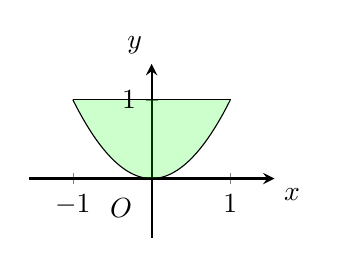
\begin{tikzpicture}
    \begin{axis}[standard,
            xtick={-1,1},
            ytick={1},
            samples=1000,
            xlabel={$x$},
            ylabel={$y$},
            xmin=-1.2,xmax=1.2,
            ymin=-0.5,ymax=1.2,
            x=1cm,
            y=1cm/1
           ]
\node[anchor=center,label=south west:$O$] at (axis cs:0,0){};
\addplot[name path=F,domain={-1:1}]{x^2};
\addplot[name path=G,domain={-1:1}]{1};
\addplot[fill=green, fill opacity=0.2] fill between [of=F and G,soft clip={domain=-1:1}];
    \end{axis}
    \end{tikzpicture}
}
\end{center}
In terms of $x$, our lower bound for $y$ is $y=x^2$ and our upper bound for $y$ is $y=1$. Our lower bound for 
$x$ is $x=-1$ and our upper bound for $x$ is $x=1$.

For $M$,
\begin{align*}
    M&=\int_{-1}^1\int_{x^2}^1 y+1\,dy\,dx\\
    &=\int_{-1}^1\lrb{\frac{1}{2}y^2+y}_{x^2}^1\,dx\\
    &=\int_{-1}^1 \lrp{\frac{1}{2}+1}-\lrp{\frac{1}{2}x^4+x^2}\,dx\\
    &=\int_{-1}^1 \frac{3}{2}-\frac{1}{2}x^4-x^2\,dx\\
    &=\lrb{\frac{3}{2}x-\frac{1}{10}x^5-\frac{1}{3}x^3}_{-1}^1\\
    &=\lrp{\frac{3}{2}-\frac{1}{10}-\frac{1}{3}}-\lrp{-\frac{3}{2}+\frac{1}{10}+\frac{1}{3}}\\
    &=\frac{32}{15}\tag{use a calculator for this :)}
\end{align*}
For $M_x$,

Our region bounds are the same as the region bounds for $M$.
\begin{align*}
    M_x&=\int_{-1}^1\int_{x^2}^1 y(y+1)\,dy\,dx\\
    &=\int_{-1}^1\int_{x^2}^1 y^2+y\,dy\,dx\\
    &=\int_{-1}^1\lrb{\frac{1}{3}y^3+\frac{1}{2}y^2}_{x^2}^1\,dx\\
    &=\int_{-1}^1 \lrp{\frac{1}{3}+\frac{1}{2}}-\lrp{\frac{1}{3}x^6+\frac{1}{2}x^4}\,dx\\
    &=\int_{-1}^1 \frac{5}{6}-\frac{1}{3}x^6-\frac{1}{2}x^4\,dx\\
    &=\lrb{\frac{5}{6}x-\frac{1}{21}x^7-\frac{1}{10}x^5}_{-1}^1\\
    &=\lrp{\frac{5}{6}-\frac{1}{21}-\frac{1}{10}}-\lrp{-\frac{5}{6}+\frac{1}{21}+\frac{1}{10}}\\
    &=\frac{48}{35}\tag{use a calculator for this :)}
\end{align*}
For $M_y$,

The region bounds will remain the same as the region bounds for $M$.
\begin{align*}
    M_y&=\int_{-1}^1\int_{x^2}^1 x(y+1)\,dy\,dx\\
    &=\int_{-1}^1\int_{x^2}^1 xy+x\,dy\,dx\\
    &=\int_{-1}^1 \lrb{\frac{1}{2}xy^2+xy}_{x^2}^1\,dx\\
    &=\int_{-1}^1 \lrp{\frac{1}{2}x+x}-\lrp{\frac{1}{2}x(x^4)+x^3}\,dx\\
    &=\int_{-1}^1 \frac{3}{2}x-\frac{1}{2}x^5-x^3\,dx\\
    &=\lrb{\frac{3}{4}x^2-\frac{1}{12}x^6-\frac{1}{4}x^4}_{-1}^1\\
    &=\lrp{\frac{3}{4}-\frac{1}{2}-\frac{1}{4}}-\lrp{\frac{3}{4}-\frac{1}{2}-\frac{1}{4}}\\
    &=0
\end{align*}
Our final answer is
\begin{subequations}
    \begin{empheq}[box=\widefbox]{align}
        \overline{x}&=\frac{M_y}{M}=\frac{0}{\frac{32}{15}}=0\nonumber\\
        \overline{y}&=\frac{M_x}{M}=\frac{\frac{48}{35}}{\frac{32}{15}}=\frac{9}{14}\nonumber\\
        \text{center of mass:}&
        \lrp{0,\frac{9}{14}}\nonumber
    \end{empheq}
\end{subequations}
\textbf{(c)} The solid in the first octant bounded by the coordinate planes and the plane $x + y + z = 2$ if the density is $\delta(x,y,z) = 2x$.

\Solution

Let's draw this from a front view and a top view. 
For the front view, we know that our $z$ is bounded below by $z=0$ since we're in the first octant. The plane $x+y+z=2$ bounds us from above.

For the top view, let's look at what happens at $z=0$. When $z=0$, $x+y+0=2$. Don't forget that we're in the first octant, so $x,y\geq 0$.
\begin{figure}[h]
\centering
\begin{minipage}{.5\textwidth}
  \centering
  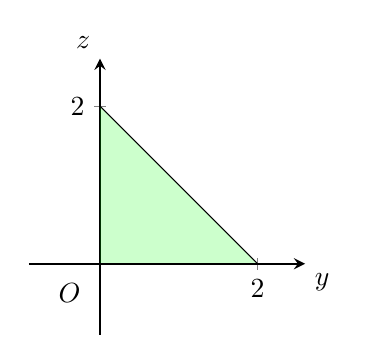
\begin{tikzpicture}
    \begin{axis}[standard,
            xtick={2},
            ytick={2},
            samples=1000,
            xlabel={$y$},
            ylabel={$z$},
            xmin=-0.5,xmax=2.2,
            ymin=-.5,ymax=2.2,
            x=1cm,
            y=1cm/1,
           ]
\node[anchor=center,label=south west:$O$] at (axis cs:0,0){};
\addplot[name path=F,domain={0:2}]{2-x};
\addplot[name path=G,domain={0:2}]{0};
\addplot[fill=green, fill opacity=0.2] fill between [of=F and G, soft clip={domain=0:2}];
    \end{axis}
    \end{tikzpicture}
  \caption*{front view when $x=0$}
  \label{fig:test1}
\end{minipage}%
\begin{minipage}{.5\textwidth}
  \centering
  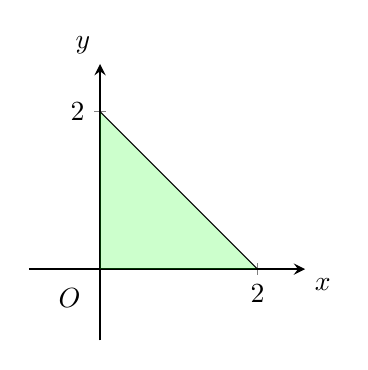
\begin{tikzpicture}
    \begin{axis}[standard,
            xtick={2},
            ytick={2},
            samples=1000,
            xlabel={$x$},
            ylabel={$y$},
            xmin=-0.5,xmax=2.2,
            ymin=-.5,ymax=2.2,
            x=1cm,
            y=1cm/1,
           ]
\node[anchor=center,label=south west:$O$] at (axis cs:0,0){};
\addplot[name path=F,domain={0:2}]{2-x};
\addplot[name path=G,domain={0:2}]{0};
\addplot[fill=green, fill opacity=0.2] fill between [of=F and G, soft clip={domain=0:2}];
    \end{axis}
    \end{tikzpicture}
  \caption*{top view}
  \label{fig:test2}
\end{minipage}
\end{figure}
All together, our region is
\begin{align*}
    0\leq &z \leq 2-x-y\\
    0 \leq &y\leq 2-x\\
    0\leq &x\leq 2
\end{align*}
For $M$,
\begin{align*}
    M&=\int_0^2\int_0^{2-x}\int_0^{2-x-y}2x\,dz\,dy\,dx\\
    &=\int_0^2\int_0^{2-x}\lrb{2xz}_0^{2-x-y}\,dy\,dx\\
    &=\int_0^2\int_0^{2-x} 2x(2-x-y)\,dy\,dx\\
    &=\int_0^2\int_0^{2-x} 4x-2x^2-2xy\,dy\,dx\\
    &=\int_0^2 \lrb{4xy-2x^2y-xy^2}_0^{2-x}\,dx\\
    &=\int_0^2 4x(2-x)-2x^2(2-x)-x(2-x)^2\,dx\\
    &=\int_0^2 x^3 - 4x^2 +4x\,dx\tag{lots of algebra here...}\\
    &=\lrb{\frac{1}{4}x^4-\frac{4}{3}x^3+2x^2}_0^2\\
    &=\frac{1}{4}(2)^2-\frac{4}{3}(2)^3+2(2)^2\\
    &=\frac{4}{3}
\end{align*}
For $M_{xy}$,

Our region bounds are the same as the region bounds for $M$.
\begin{align*}
    M_{xy}&=\int_0^2\int_0^{2-x}\int_0^{2-x-y} z(2x)\,dz\,dy\,dx\\
    &=\int_0^2\int_0^{2-x}\lrb{xz^2}_0^{2-x-y}\,dy\,dx\\
    &=\int_0^2 \int_0^{2-x}x(2-x-y)^2\,dy\,dx\\
    &=\int_0^2\lrb{-\frac{1}{3}x(2-x-y)^3}_0^{2-x}\,dx\\
    &=-\frac{1}{3}\int_0^2 -x(2-x)^3\,dx\\
    &=\frac{1}{3}\int_0^2 x (2-x)^3\,dx\\
    &u=2-x\hspace{2em}du=-dx\\
    &u(0)=2\hspace{2em}u(2)=0\\
    &-\frac{1}{3}\int_2^0 (2-u)u^3\,du\\
    &=\frac{1}{3}\int_0^2 2u^3-u^4\,du\\
    &=\frac{1}{3}\lrb{\frac{1}{2}u^4-\frac{1}{5}u^5}_0^2\\
    &=\frac{1}{3}\lrp{8-\frac{32}{5}}\\
    &=\frac{8}{15}
\end{align*}
For $M_{yz}$,

Our region bounds are the same as the region bounds for $M$.
\begin{align*}
    \int_0^2\int_0^{2-x}\int_0^{2-x-y}x(2x)\,dz\,dy\,dx\\
    &=\int_0^2\int_0^{2-x}\lrb{2x^2z}_0^{2-x-y}\,dy\,dx\\
    &=\int_0^2\int_0^{2-x} 2x^2(2-x-y)\,dy\,dx\\
    &=\int_0^2\lrb{-x^2(2-x-y)^2}_0^{2-x}\,dx\\
    &=\int_0^2 x^2(2-x)^2\,dx\\
    &=\int_0^2 x^2(4-4x+x^2)\,dx\\
    &=\int_0^2 4x^2 -4x^3 + x^4\,dx\\
    &=\lrb{\frac{4}{3}x^3-x^4+\frac{1}{5}x^5}_0^2\\
    &=\frac{16}{15}
\end{align*}

For $M_{xz}$,

By symmetry, $M_{xz}=M_{xy}=\dfrac{8}{15}$.

Alternatively, you could solve the integral
\begin{align*}
     \int_0^2\int_0^{2-x}\int_0^{2-x-y} y(2x)\,dz\,dy\,dx
\end{align*}
which is super time consuming :)

Our final answer is
\begin{subequations}
    \begin{empheq}[box=\widefbox]{align}
        \overline{x}&=\frac{M_{yz}}{M}=\frac{\frac{16}{15}}{\frac{4}{3}}=\frac{4}{5}\nonumber\\
        \overline{y}&=\frac{M_{xz}}{M}=\frac{\frac{8}{15}}{\frac{4}{3}}=\frac{2}{5}\nonumber\\
        \overline{z}&=\frac{M_{xy}}{M}=\frac{\frac{8}{15}}{\frac{4}{3}}=\frac{2}{5}\nonumber\\
        \text{center of mass:}&
        \lrp{\frac{4}{5},\frac{2}{5},\frac{2}{5}}\nonumber
    \end{empheq}
\end{subequations}

\textbf{(d)} A solid cube in the first octant bounded by the coordinate planes and by the
planes $x = 1$, $y = 1$, and $z = 1$ if the density is $\delta(x,y,z) = x + y + z + 1$.

\Solution

This region is literally a cube in the first octant, so our bounds are
\begin{align*}
    0\leq &z\leq 1\\
    0\leq &y\leq 1\\
    0\leq &x\leq 1
\end{align*}
For $M$,
\begin{align*}
    M&=\int_0^1\int_0^1\int_0^1 x+y+z+1\,dz\,dy\,dx\\
    &=\int_0^1\int_0^1\lrb{xz+yz+\frac{1}{2}z^2+z}_0^1\,dy\,dx\\
    &=\int_0^1\int_0^1 x+y+\frac{1}{2}+1\,dy\,dx\\
    &=\int_0^1 \lrb{xy+\frac{1}{2}y^2+\frac{1}{2}y+y}_0^1\,dx\\
    &=\int_0^1 x +\frac{1}{2}+\frac{1}{2}+1\,dx\\
    &=\lrb{\frac{1}{2}x^2+\frac{1}{2}x+\frac{1}{2}x+x}_0^1\\
    &=\frac{5}{2}
\end{align*}

For $M_{xy}$,

Our region bounds are the same as the region bounds for $M$.
\begin{align*}
    M_{xy}&=\int_0^1\int_0^1\int_0^1 z(x+y+z+1)\,dz\,dy\,dx\\
    &=\int_0^1\int_0^1\int_0^1 xz+yz+z^2+z\,dz\,dy\,dx\\
    &=\int_0^1\int_0^1\lrb{\frac{1}{2}xz^2+\frac{1}{2}yz^2+\frac{1}{3}z^3+\frac{1}{2}z^2}_0^1\,dy\,dx\\
    &=\int_0^1\int_0^1 \frac{1}{2}x+\frac{1}{2}y+\frac{1}{3}+\frac{1}{2}\,dy\,dx\\
    &=\int_0^1\lrb{\frac{1}{2}xy+\frac{1}{4}y^2+\frac{1}{3}y+\frac{1}{2}y}_0^1\,dx\\
    &=\int_0^1 \frac{1}{2}x+\frac{1}{4}+\frac{1}{3}+\frac{1}{2}\,dx\\
    &=\lrb{\frac{1}{4}x^2+\frac{1}{4}x+\frac{1}{3}x+\frac{1}{2}x}_0^1\\
    &=\frac{4}{3}\tag{use your calculator :)}
\end{align*}
Since our region is a cube, by symmetry, $M_{xy}=M_{yz}=M_{xz}$. If you don't believe me, you can go through the pain and suffering of calculating the integrals yourself :)

Our final answer is
\begin{subequations}
    \begin{empheq}[box=\widefbox]{align}
        \overline{x}&=\frac{M_{yz}}{M}=\frac{\frac{4}{3}}{\frac{5}{2}}=\frac{8}{15}\nonumber\\
        \overline{y}&=\frac{M_{xz}}{M}=\frac{\frac{4}{3}}{\frac{5}{2}}=\frac{8}{15}\nonumber\\
        \overline{z}&=\frac{M_{xy}}{M}=\frac{\frac{4}{3}}{\frac{5}{2}}=\frac{8}{15}\nonumber\\
        \text{center of mass:}&
        \lrp{\frac{8}{15},\frac{8}{15},\frac{8}{15}}\nonumber
    \end{empheq}
\end{subequations}

\textbf{Problem 4}

Find the centroid of the solid bounded below by $z = 4y^2$, above by the plane $z = 4$, and on the ends by the planes $x = 1$ and $x = -1$.

\Solution

For $M$,

Our lower bound for $z$ is $z=4y^2$ and our upper bounds for $z$ is $z=4$. Our lower bound for $x$ is $x=-1$ and our upper bound for $x$ is $x=1$. We can get our bounds for $y$ by setting $z=4y^2$ and $z=4$ equal to each other.
\begin{align*}
    4y^2&=4\\
    y^2&=1\\
    y&=\pm 1
\end{align*}
Now, we can solve for our $M$.
\begin{align*}
    M&=\int_{-1}^1\int_{-1}^1\int_{4y^2}^4\,dz\,dy\,dx\\
    &=\int_{-1}^1\int_{-1}^1\lrb{z}_{4y^2}^4\,dy\,dx\\
    &=\int_{-1}^1\int_{-1}^1 4-4y^2\,dy\,dx\\
    &=\int_{-1}^1 \lrb{4y-\frac{4}{3}y^3}_{-1}^1\,dx\\
    &=\int_{-1}^1 \frac{16}{3}\,dx\\
    &=\lrb{\frac{16}{3}x}_{-1}^1\\
    &=\frac{32}{3}
\end{align*}
By symmetry, $\overline{x}=\overline{y}=0$. We just need to find $\overline{z}$ by getting $M_{xy}$.

For $M_{xy}$,

The region bounds would be the same as the region bounds for $M$.
\begin{align*}
    M_{xy}&=\int_{-1}^1\int_{-1}^1\int_{4y^2}^4z\, dz\,dy\,dx\\
    &=\int_{-1}^1\int_{-1}^1 \lrb{\frac{1}{2}z^2}_{4y^2}^{4}\,dy\,dx\\
    &=\int_{-1}^1\int_{-1}^1 8-8y^4\,dy\,dx\\
    &=\int_{-1}^1\lrb{8y-\frac{8}{5}y^5}_{-1}^1\,dx\\
    &=\int_{-1}^1 \frac{64}{5}\,dx\\
    &=\lrb{\frac{64}{5}x}_{-1}^1\\
    &=\frac{128}{5}
\end{align*}
Our final answer is
\begin{subequations}
    \begin{empheq}[box=\widefbox]{align}
        \overline{x}&=0\nonumber\\
        \overline{y}&=0\nonumber\\
        \overline{z}&=\frac{M_{xy}}{M}=\frac{\frac{128}{5}}{\frac{32}{3}}\nonumber\\
        \text{center of mass:}&
        \lrp{0,0,\frac{12}{5}}\nonumber
    \end{empheq}
\end{subequations}
\textbf{Problem 5}

Consider the solid bounded below by the paraboloid $z = x^2+ y^2$ and above by the plane $z = 4$.

\textbf{(a)} Find the centroid of the solid.

\Solution

As stated in the problem, the solid is bounded below by the parabolid $z=x^2+y^2$ and above by the plane $z=4$. The top view would be $4=x^2+y^2$, a circle with radius $2$.

In terms of $x$, the lower bound of $y$ would be $y=-\sqrt{4-x^2}$ and the upper bound would be $y=\sqrt{4-x^2}$. The lower bound of $x$ would be $x=-2$ and the upper bound would be $x=2$.

All together, our bounds are
\begin{align*}
    x^2+y^2\leq &z \leq 4\\
    -\sqrt{4-x^2}\leq &y\leq \sqrt{4-x^2}\\
    -2\leq &x\leq 2
\end{align*}
For $M$,
\begin{align*}
    M&=\int_{-2}^2\int_{-\sqrt{4-x^2}}^{\sqrt{4-x^2}}\int_{x^2+y^2}^4 \,dz\,dy\,dx\\
    &=\int_{-2}^2\int_{-\sqrt{4-x^2}}^{\sqrt{4-x^2}}\lrb{z}_{x^2+y^2}^4\,dy\,dx\\
    &=\int_{-2}^2\int_{-\sqrt{4-x^2}}^{\sqrt{4-x^2}} 4-(x^2+y^2)\,dy\,dx
\end{align*}
Now we could do this in Cartesian, but let's do this in polar instead.

Since we are integrating the full circle, our $\theta$ will go from $0$ to $2\pi$. Our $r$ will go from $0$ to $2$.
\begin{align*}
    \int_{-2}^2\int_{-\sqrt{4-x^2}}^{\sqrt{4-x^2}} 4-(x^2+y^2)\,dy\,dx&=\int_0^{2\pi}\int_0^2 (4-r^2)r\,dr\,d\theta\tag{in polar, $x^2+y^2=r^2$}\\
    &=\int_0^{2\pi}\int_0^2 4r-r^3\,d\theta\\
    &=\int_0^{2\pi} \lrb{2r^2-\frac{1}{4}r^4}_0^2]\,d\theta\\
    &=\int_0^{2\pi} 4\,d\theta\\
    &=\lrb{4\theta}_0^{2\pi}\\
    &=8\pi
\end{align*}
By symmetry, $\overline{x}=\overline{y}=0$. We'll just need to find $M_{xy}$ to get our $\overline{z}$.

For $M_{xy}$,

The region bounds would be the same as the region bounds for $M$.
\begin{align*}
    M_{xy}&=\int_{-2}^2\int_{-\sqrt{4-x^2}}^{\sqrt{4-x^2}}\int_{x^2+y^2}^4 z\,dz\,dy\,dx\\
    &=\int_{-2}^2\int_{-\sqrt{4-x^2}}^{\sqrt{4-x^2}}\lrb{\frac{1}{2}z^2}_{x^2+y^2}^4\,dy\,dx\\
    &=\int_{-2}^2\int_{-\sqrt{4-x^2}}^{\sqrt{4-x^2}} 8-\frac{1}{2}(x^2+y^2)^2\,dy\,dx\\
    &=\int_0^{2\pi}\int_{0}^2 (8-\frac{1}{2}(r^2)^2)r\,dr\,d\theta\tag{let's change to polar :)}\\
    &=\int_0^{2\pi}\int_0^2 8r-\frac{1}{2}r^5\,dr\,d\theta\\
    &=\int_0^{2\pi}\lrb{4r^2-\frac{1}{12}r^6}_0^2\,d\theta\\
    &=\int_0^{2\pi} 16 -\frac{64}{12}\,d\theta\\
    &=\lrb{16\theta-\frac{64}{12}\theta}_0^{2\pi}\\
    &=\frac{64\pi}{3}
\end{align*}
Our final answer is
\begin{subequations}
    \begin{empheq}[box=\widefbox]{align}
        \overline{x}&=0\nonumber\\
        \overline{y}&=0\nonumber\\
        \overline{z}&=\frac{M_{xy}}{M}=\frac{\frac{64\pi}{3}}{8\pi}=\frac{8}{3}\nonumber\\
        \text{center of mass:}&
        \lrp{0,0,\frac{8}{3}}\nonumber
    \end{empheq}
\end{subequations}
\textbf{(b)} Find the plane $z = c$ that divides the solid into two parts of equal volume. (This plane does not pass through the centroid.)

\Solution

For the plane $z=c$ to divide the solid into two parts of equal volume, the volume $M$ bounded below by the plane $x^2+y^2$ and bounded above by $z=c$ must equal half of the $M$ we found in \textbf{(a)} which would be $4\pi$.

Our top view would be $c=x^2+y^2$, a circle with radius $\sqrt{c}$.

All together, our bounds are
\begin{align*}
    x^2+y^2\leq &z \leq c\\
    -\sqrt{c-x^2}\leq &y\leq \sqrt{c-x^2}\\
    -\sqrt{c}\leq &x\leq\sqrt{c}
\end{align*}
For $M$,
\begin{align*}
    M=4\pi&=\int_{-\sqrt{c}}^{\sqrt{c}}\int_{-\sqrt{c-x^2}}^{\sqrt{c-x^2}}\int_{x^2+y^2}^c\,dz\,dy\,dx\\
    &=\int_{-\sqrt{c}}^{\sqrt{c}}\int_{-\sqrt{c-x^2}}^{\sqrt{c-x^2}}\lrb{z}_{x^2+y^2}^c\,dy\,dx\\
    &=\int_{-\sqrt{c}}^{\sqrt{c}}\int_{-\sqrt{c-x^2}}^{\sqrt{c-x^2}} c-(x^2+y^2)\,dy\,dx\\
    &=\int_0^{2\pi}\int_0^{\sqrt{c}} (c-r^2)r\,dr\,d\theta\tag{let's convert to polar}\\
    &=\int_0^{2\pi}\int_0^{\sqrt{c}} cr-r^3\,dr\,d\theta\\
    &=\int_0^{2\pi}\lrb{\frac{1}{2}cr^2-\frac{1}{4}r^4}_0^{\sqrt{c}}\,d\theta\\
    &=\int_0^{2\pi} \frac{1}{2}c^2-\frac{1}{4}c^2\,d\theta\\
    &=\lrb{\frac{1}{2}c^2\theta-\frac{1}{4}c^2\theta}_0^{2\pi}\\
    &=\frac{1}{2}c^2(2\pi)-\frac{1}{4}c^2(2\pi)\\
    &=\frac{1}{2}c^2\pi
\end{align*}
Since we know $M=4\pi$,
\begin{align*}
    4\pi&=\frac{1}{2}c^2\pi\\
    8&=c^2\\
    c&=\pm 2\sqrt{2}
\end{align*}
However, we know that $c$ must be between $0$ and $4$ since $z=c$ is supposed to be a plane to divide the solid bounded by planes $z=4y^2$ and $z=4$.

Therefore, $c=2\sqrt{2}$.\qed
\end{document}